\chapter{用户态协议栈的兼容性设计}

本章将用两节来对该用户态协议栈的设计进行详细阐述,第一节将从整体层面介绍用户态协议栈的架构,包括协议栈前后端分离的设计以及主要模块的分工、协议栈与网络应用进程间通信等。第二节从兼容性方面对协议栈的各种设计进行详细介绍,这也是该用户态协议栈最大的贡献与意义,其中包括POSIX网络系统调用接口的劫持、文件描述符空间的分割管理、Epoll IO多路复用的设计、并发流网络模型的设计、网络应用进程异常崩溃的处理机制等,通过这些设计使得该用户态协议栈在不需要修改网络应用源码的情况下就可以零成本移植,并获得网络性能的提升。

\section{协议栈整体系统设计}

用户态协议栈的兼容性的实现只有能为传统网络应用带来性能提升才会有意义,而协议栈的整体设计对整个系统的性能起到关键的作用,本节将对协议栈的整体设计进行阐述,并对其中为何这么设计的原因进行分析。
% dlsym~\cite{DLSYM}
% \cite{IO-models}
% $2^{30}$

\subsection{协议栈与应用的分核设计}

传统Linux内核网络协议栈通常是由操作系统来完成调度以及与网络应用的数据消息和控制信息的传递,而将网络协议栈搬离到用户态之后,操作系统就丧失对协议栈的绝对控制而由用户态开发人员来决定其管理与调度。用户态网络协议栈与网络应用两个执行流如何进行调度与管理成为设计之初最关键的问题,通常有两种管理方式,第一种是将协议栈执行流与网络应用执行流绑定在同一个CPU核上,比如mTCP~\cite{mTCP}就采用该种模式,此方式的优势在于减少数据跨核进行同步造成的Cache Miss,并且对CPU核资源的利用率较高,不过劣势在于协议栈执行流与网络应用执行流可能存在严重的CPU资源争抢,即使通过合理的调度机制避免CPU争夺也会存在着两种执行流在高并发高吞吐下频繁上下文切换带来的开销;第二种是将协议栈执行流与网络应用执行流分别放在两个不同的CPU核上,比如IsoStack~\cite{IsoStack}就是将协议栈处理逻辑放在专用的物理核上,该方式的好处在于可以较好地避免CPU资源的争夺,为网络协议栈收发包提供最大化的CPU资源,但其坏处是数据跨核同步带来的开销和对CPU核资源的利用率较低。本文经过实验验证,第二种方式会获得更优的网络性能,所以该协议栈采用的是将协议栈与应用分核绑定的设计。

\vspace{-10pt}
\begin{figure}[H] % use float package if you want it here
  \centering
  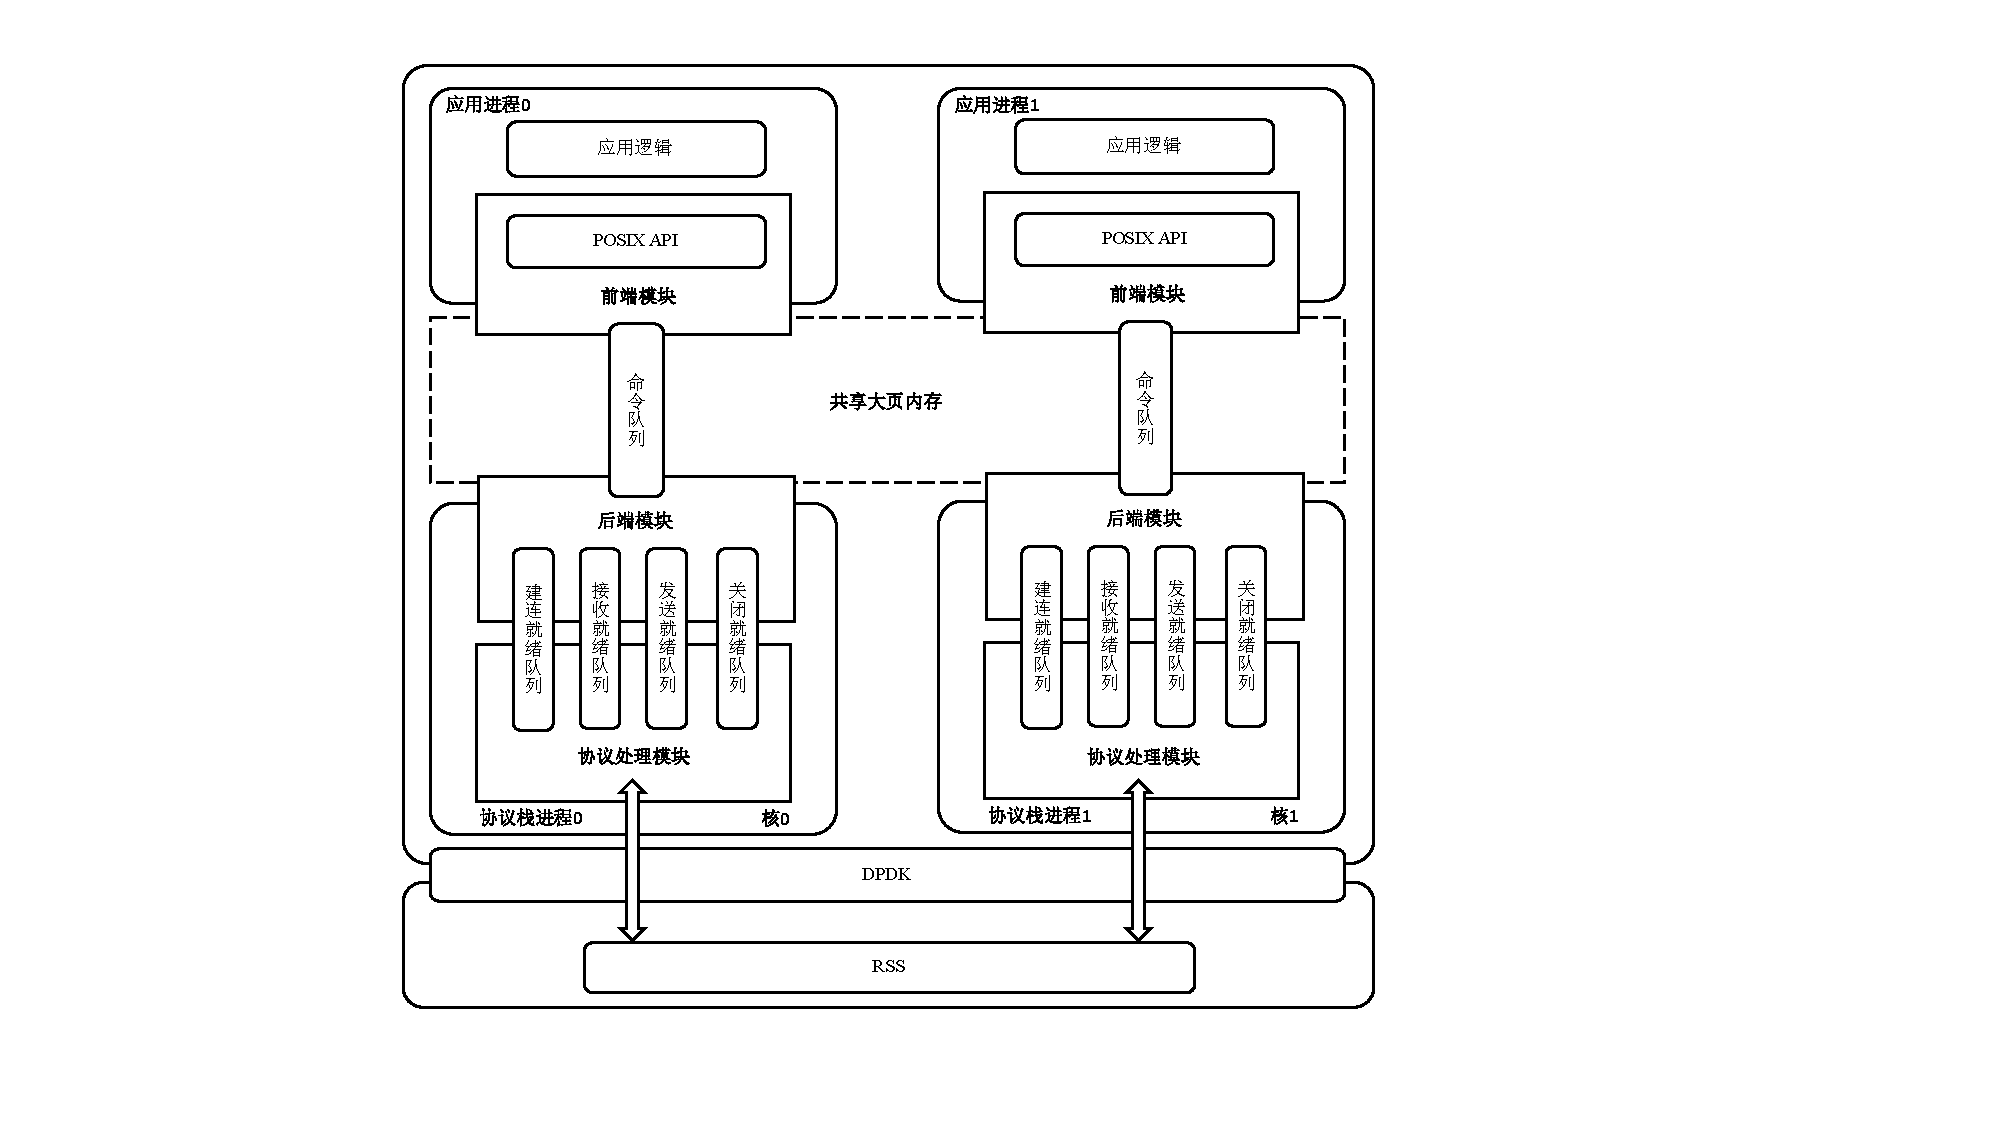
\includegraphics[width=\textwidth]{architecture}
  \caption{用户态协议栈架构图}
  \label{fig:architecture}
\end{figure}
\vspace{-10pt}

整体系统的架构图如图~\ref{fig:architecture}所示,协议栈底层使用Intel的高速IO收发包框架DPDK~\cite{DPDK},并利用RSS(Receive Side Scaling)根据接收的五元组信息和Hash算法将数据包指派到特定的CPU核上,这样该连接的所有数据包都会在该CPU核上进行处理。两个协议栈进程分别运行在两个专用的物理核上,而两者分别与对应的网络应用进程进行网络连接信息交互。网络协议栈进程由协议处理模块和后端模块组成,应用进程由前端模块和网络应用组成,前后端作为协议栈与网络应用通信的接口,基于DPDK大页内存的消息队列实现的命令队列来完成前后端通信。下面对各个主要模块进行更加详细的描述。

协议处理模块是基于Linux内核3.14.2版本中网络协议栈的代码进行剥离和二次开发,涵盖数据链路层、网络层、传输层的数据包的封装、解析、校验和状态维护。底层通过高速IO轮询收发包框架DPDK进行收发包,替代传统内核协议栈中基于中断的收包模式,减少收包硬件中断对CPU的压力。在接收方向,DPDK通过RSS技术根据对称哈希算法和五元组信息对数据包进行分配到相应的网卡队列上,接下来数据包被DPDK网卡驱动模块提供的收包函数接收到指定的协议栈进程核中,从而进入用户态数据链路层的逻辑处理以及后续的TCP状态转移,并将新建连接、读写和关闭等网络事件传送到对应的就绪队列。在发送端,DPDK根据对称哈希算法将该连接的响应报文传递到接收时的网卡队列中,从而发送给客户端。这样一个完整TCP连接的数据包的网络逻辑处理都是在同一个网卡队列、CPU核上进行处理,有利于协议栈的多核扩展性。

后端模块是整个系统大页内存、关键数据结构等各种资源的管理中心。在协议栈进程初始化时,后端init函数会对用户态套接字、文件描述符资源等资源预分配,默认socket的最大并发数是2048,该最大并发数可满足绝大部分的网络应用使用场景。这些申请到的套接字和文件描述符资源以资源池的形式通过DPDK提供的无锁循环队列rte\_ring以生产者消费者模型为后续新建连接提供相应资源,并在连接断开时候将套接字和文件描述符资源进行回收,防止其发生内存泄漏。在协议栈进程初始化时还会对新建连接就绪队列、接收就绪队列、发送就绪队列、关闭就绪队列进行初始化。当协议栈完成初始化后,就进入不断地循环读取数据包、从就绪队列中读取网络事件以及处理从前端传来的网络函数调用命令,并进行相应命令的后端网络逻辑处理。当读取到新建连接或有socket新数据到来时候,就会进行FIFO写操作从而唤醒前端的内核epoll\_wait,并同时将相应的socket fd以及事件传送到前后端共享的缓冲队列中。

前端模块作为用户态协议栈最终暴露给网络应用的部分,是用户态协议栈实现高度兼容性的关键模块,其向上给应用提供与POSIX API完全一样的网络接口,这是通过LD\_PRELOAD环境变量以及动态链接技术来完成。在网络应用调用socket、read、write等函数后产生相应的命令,并放入命令队列中。此外,前端在创建Epoll结构体时,并通过内核Epoll监听额外创建的FIFO,一旦后端有事件待前端响应便进行FIFO写从而唤醒前端内核epoll\_wait调用,从而完成前端监听事件的唤醒,网络应用可以进行下一步的socket读写或新连接的建立。此外,由于用户态协议栈对POSIX网络系统调用read、epoll\_wait等进行了劫持,并且这些函数的输入参数的文件描述符可能是非网络fd,前端模块还负责对协议栈管理的网络文件描述符与内核管理的非网络文件描述符进行分割管理。当网络应用调用被协议栈劫持的read函数时候,如果是对socket网络文件描述符进行读操作,则走用户态协议栈的处理逻辑;而如果判定为非网络文件描述符,比如是文件系统等,则会通过dlsym~\cite{DLSYM}间接调用内核read函数来走内核流程,这样为网络应用提供完整的网络系统调用功能。前端中的兼容性设计会在下一节进行更加详细的阐述。

\subsection{进程间通信设计}
由于该系统的协议栈进程与网络应用进程是在两个不同物理CPU核上运行,传统网络服务器在高并发高吞吐的情况下会产生大量的控制消息和网络数据的传递,能否高效解决进程间通信问题就决定了能否均摊由于跨核导致的数据同步、Cache Miss等开销,对系统的整体性能尤为重要。在此,先对各种常见的进程间通信方式IPC进行简单介绍与对比,这对于为协议栈与网络应用进程间通信的抉择很有意义。

匿名管道(pipe)是操作系统早期一种进程间通信手段,数据流只能在管道中进行单向传递,只能读或者只能写,并且通信的双方只能是父子进程,这种严苛的使用条件也导致管道无法成为本系统的选择。有名管道FIFO是更高级的管道,它与pipe相比的优势在于,进程通信双方可以不具备父子关系,由于其操作起来简单方便并具备比较高的少量数据读写性能,所以FIFO被本系统用来当作后端向前端传递事件的触发通道。消息队列是一种符合先入先出原则的链表,常用来实现消费者生产者模式,并且其承载的信息格式并没有限制,可以通过结构体自定义消息格式,所以消息队列在该系统的前后端消息传递、socket和文件描述符资源管理等多处进行使用。内核中有消息队列的实现,但是由于在频繁调用的情况下系统调用的开销也不容忽视,所以本系统基于DPDK提供的无锁消息队列rte\_ring来完成进程间消息传递的。共享内存是在进程间进行数据传递最为高效的通信方式,在物理内存中的一段地址可以通过内存映射共享到不同进程的地址空间中,完成映射后的地址可以直接在不同进程中直接进行读写操作。本系统socket、文件描述符资源池就是基于DPDK大页共享内存提供的rte\_mempool来完成的。信号量本质上是一种多元互斥锁,当多个进程对同一个资源进行并发读写时候,往往需要信号量来进行多进程之间的同步。socket网络套接字是当前最为常用的进程间通信方式,分为远端机器之间的通信与本地Unix域套接字通信,后者在本系统的异常检测模块中采用。

本小节重点对协议栈与网络应用之间的进程间通信进行详细描述,网络应用在调用各种POSIX网络调用时候会将相应的指令放入命令队列中,该命令队列就是基于消息队列与共享内存来完成的,而DPDK刚好提供了一套基于CAS实现无锁化的消息队列和共享内存,即rte\_ring和rte\_mempool,两者常常需要配合使用。在协议栈初始化之时,在DPDK的primary进程中创建rte\_ring和rte\_mempool,在DPDK的secondary进程启动之后,就通过函数rte\_ring\_lookup和rte\_mempool\_lookup来获取相应的ring和mempool的内存地址,并且这些地址都是位于DPDK统一管理的大页内存中。当应用调用POSIX网络函数并产生一个相应命令后,则从mempool资源池中获取一个真实命令结构体地址,再将该地址enqueue进入命令队列rte\_ring中。当后端在轮询阶段并且命令队列中存在待处理命令,就会将其dequeue并进行该命令的后端相关操作,待完成操作之后就将该命令结构体地址返还给mempool,这样即可完成从前端向后端通信的过程。可以看出rte\_mempool类似一个资源池管理着真实的数据,而rte\_ring作为一个环形队列管理真实数据的指针。

后端在接收相应数据包或完成TCP三次握手之后需要通知阻塞在epoll\_wait的前端执行流,这就需要前端在创建epoll结构时候就为从后端到前端的信道建立一个有名管道FIFO,并且通过内核epoll完成对该有名管道可读事件的监听。当后端产生相应事件后先对该事件进行判重,防止一次同时向前端传递重复的事件,接着会将包括文件描述符、事件种类等相关信息封装后推送进事件队列,并向有名管道中写一个字节的数据,从而触发前端内核epoll\_wait返回,这样在前端获取这些待响应网络事件并结合待响应非网络事件统一返回给网络应用。这样便完成了从后端到前端的进程间通信过程。

\section{协议栈兼容性相关设计}

兼容性是本工作的研究重点,如何让网络应用在不修改任何源码几乎零成本地移植在用户态协议栈上需要在兼容性设计上做不少具有挑战性的工作。首先需要对网络服务器的经典模式熟练掌握,比如多进程one process per request类型,多进程主从类型,多线程one thread per request类型,Epoll IO多路复用模型以及与多进程、多线程的结合,此外还需要对Nginx、Lighttpd、Redis等主流网络应用的源码及其相关POSIX API进行充分调研与了解,这些工作是实现网络应用高度兼容性的前提。在这些工作的基础上就是技术上对兼容性的设计与实现,本节将从POSIX网络API的劫持、文件描述符空间的分割与管理、用户态Epoll IO多路复用机制、并发流网络模型的设计和系统异常检测机制展开进行阐述。

\subsection{POSIX网络API的劫持}

内核网络协议栈的实现有Linux、FreeBSD、Solaris等各种版本,但它们都统一遵循IEEE最初主导的POSIX(Portable Operating System Interface of UNIX)规范,该协议规定了操作系统为上层应用提供接口的标准,其中包含socket网络编程这套函数接口,这样做的好处是完全按照POSIX规范编写的应用程序可以跨Unix各种操作系统版本直接运行,所以传统网络应用基本都是遵循POSIX规范进行编写。而想要实现传统网络应用不修改任何源码的移植成本,就必须对POSIX网络API进行劫持。如图~\ref{fig:hijack}显示传统网络应用不调用内核操作系统的网络系统调用,即Linux的Glibc库,而去调用用户态协议栈提供的一套命名完全一样的网络接口。

\vspace{-10pt}
\begin{figure}[H] % use float package if you want it here
  \centering
  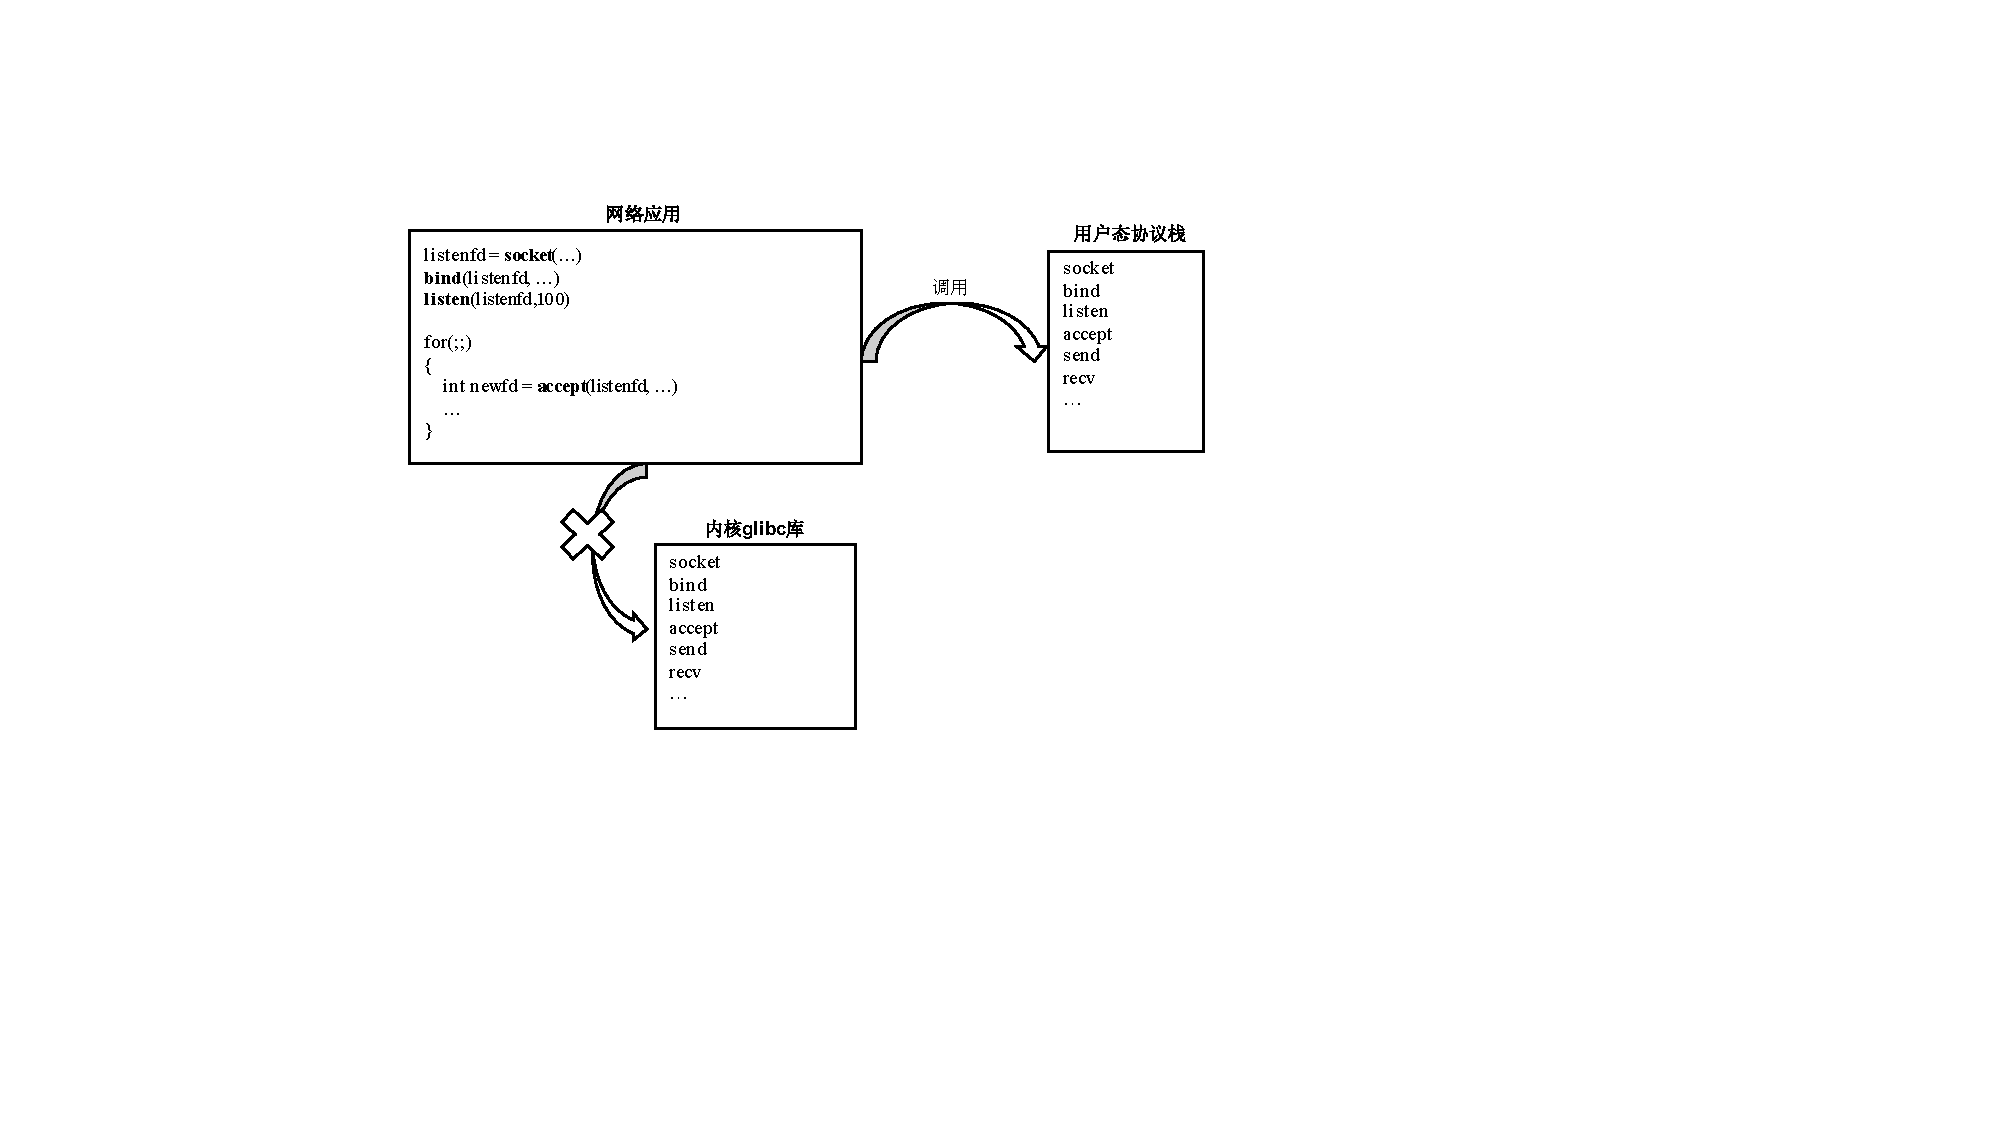
\includegraphics[width=\textwidth]{hijack}
  \caption{网络应用调用关系图}
  \label{fig:hijack}
\end{figure}
\vspace{-10pt}

本系统是在Linux环境中进行实现,而Linux中的系统调用封装成的Glibc是以动态链接库的形式被网络应用加载。动态链接相比静态链接的优势在于动态库仅需要加载到物理内存一次就可以被多个进程通过内存映射共享到其进程地址空间从而大大节约物理内存资源。本设计的劫持关键技术使用LD\_PRELOAD环境变量,它的作用是修改程序运行时加载动态链接库的优先级,尤其当两个动态库中含有命名完全相同的函数时。整体劫持方案如图~\ref{fig:hijack_impl}所示,首先通过userspace\_stack.c对用户态协议栈的函数重新封装成与POSIX接口完全一样,并将其用gcc编译成动态链接库stack.so。在运行网络应用可执行文件时将stack.so文件存放到环境变量LD\_PRELOAD中,这意味着stack.so动态库的加载优先级高于POSIX系统调用动态库libc.so。当传统网络应用在运行至网络API时,首先会先加载Linux系统中的ld.so动态连接器,它是进程加载其他链接库的桥梁,接下来会直接调用stack.so动态库中网络函数的实现;而当传统网络应用调用非网络API时,依然会调用libc.so中的内核系统调用。但是read、epoll\_wait等相关API的实现依然需要借助内核read、epoll\_wait来实现阻塞或磁盘文件IO等操作,所以stack.so又通过dlsym运行时动态链接技术对内核进行间接调用,并将其命名为kernel\_xxx以便区分,这会在文件描述符空间管理和Epoll多路复用设计小节中详细描述。

LD\_PRELOAD来实现网络系统调用的劫持几乎没有性能损耗,并且该方案对Apache网络服务器通过其他网络库间接调用glibc动态库的模式依然有效,当然这种方式目前只能对调用POSIX API且C语言实现的传统网络应用有效,至于最新基于golang等语言的网络服务并不在本工作的考虑范围之内。

\vspace{-10pt}
\begin{figure}[H] % use float package if you want it here
  \centering
  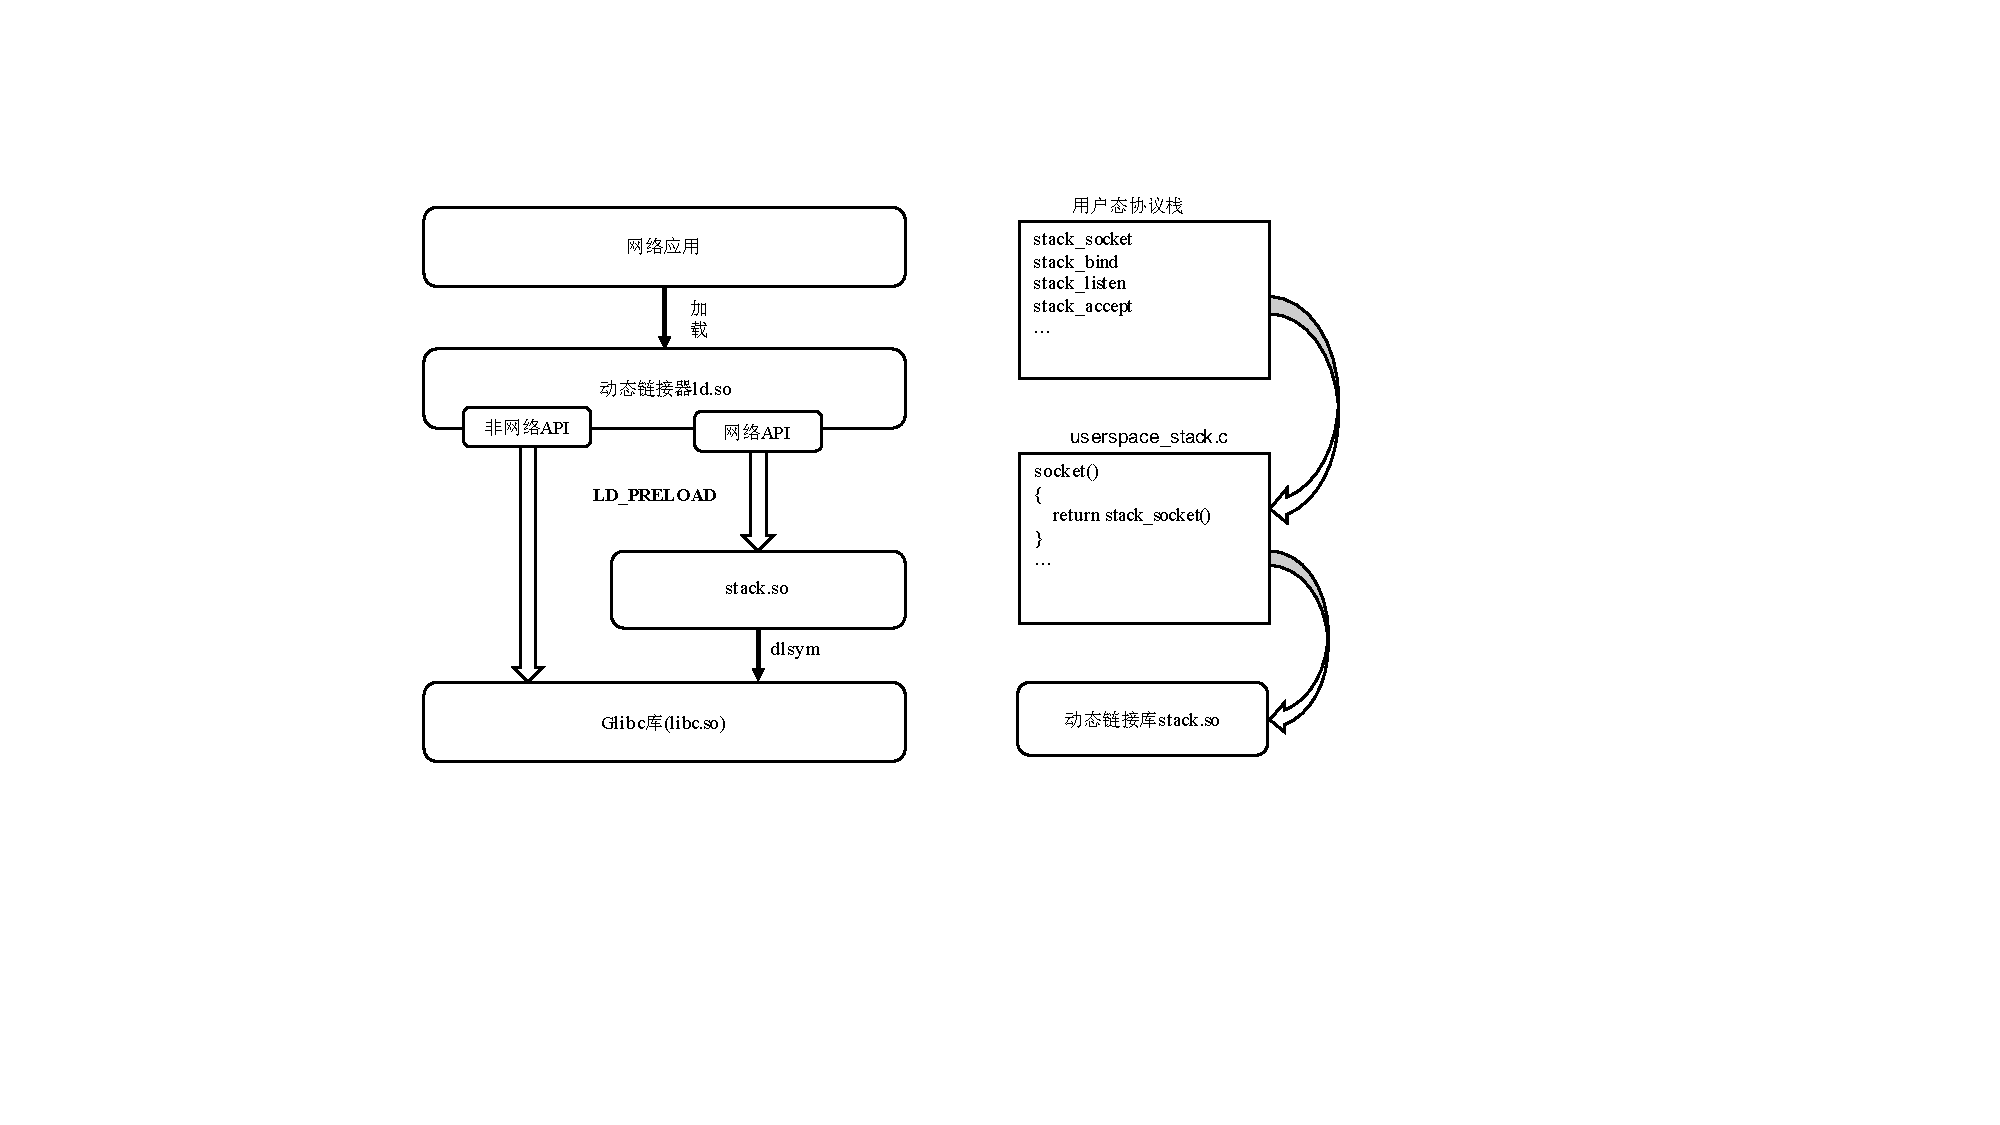
\includegraphics[width=\textwidth]{hijack_impl}
  \caption{劫持POSIX网络API设计图}
  \label{fig:hijack_impl}
\end{figure}
\vspace{-10pt}

\subsection{文件描述符FD空间的管理}

劫持POSIX网络相关API引入一个新的问题,那就是read、epoll\_wait等函数参数中的文件描述符可能并不只是socket网络文件描述符,比如读写一个磁盘文件或epoll监听一个有名管道等,而用户态协议栈仅实现了操作系统中TCP/IP协议栈功能,并不对非网络功能进行支持。所以在传统应用调用被用户态协议栈劫持的read等函数之后,就需要先对文件描述符进行分割管理,对socket网络文件描述符运行用户态协议栈处理逻辑,而非网络文件描述符依然调用内核kernel\_read函数,这也是stack.so文件依然需要使用dlsym对内核系统调用进行链接的原因。

由于文件描述符是有符号型整数,最简单的实现方案就是将文件描述符整数空间一分为二,如图~\ref{fig:split_fd1}所示,以$2^{30}$作为分界点,从左向右为非网络文件描述符并调用内核系统调用。而如果是socket网络文件描述符则根据$2^{31}-1 - fd$重映射到右边大整数的空间。这样传入的文件描述符如果不小于$2^{30}$则判定为socket网络文件描述符,并走用户态协议栈逻辑,而如果小于$2^{30}$则为非网络文件描述符并进行内核系统调用。由于在实际百万级高网络并发的条件下,socket连接数也远小于$2^{30}$,所以该方案理论上是可行的,并且本文初期就采用该方案成功移植Nginx网络应用。然而在Lighttpd、Redis等网络应用中常常需要将socket文件描述符作为数组下标,该方案返回的socket文件描述符过大必然会造成数组越界访问,从而引发系统崩溃。

\vspace{-10pt}
\begin{figure}[H] % use float package if you want it here
  \centering
  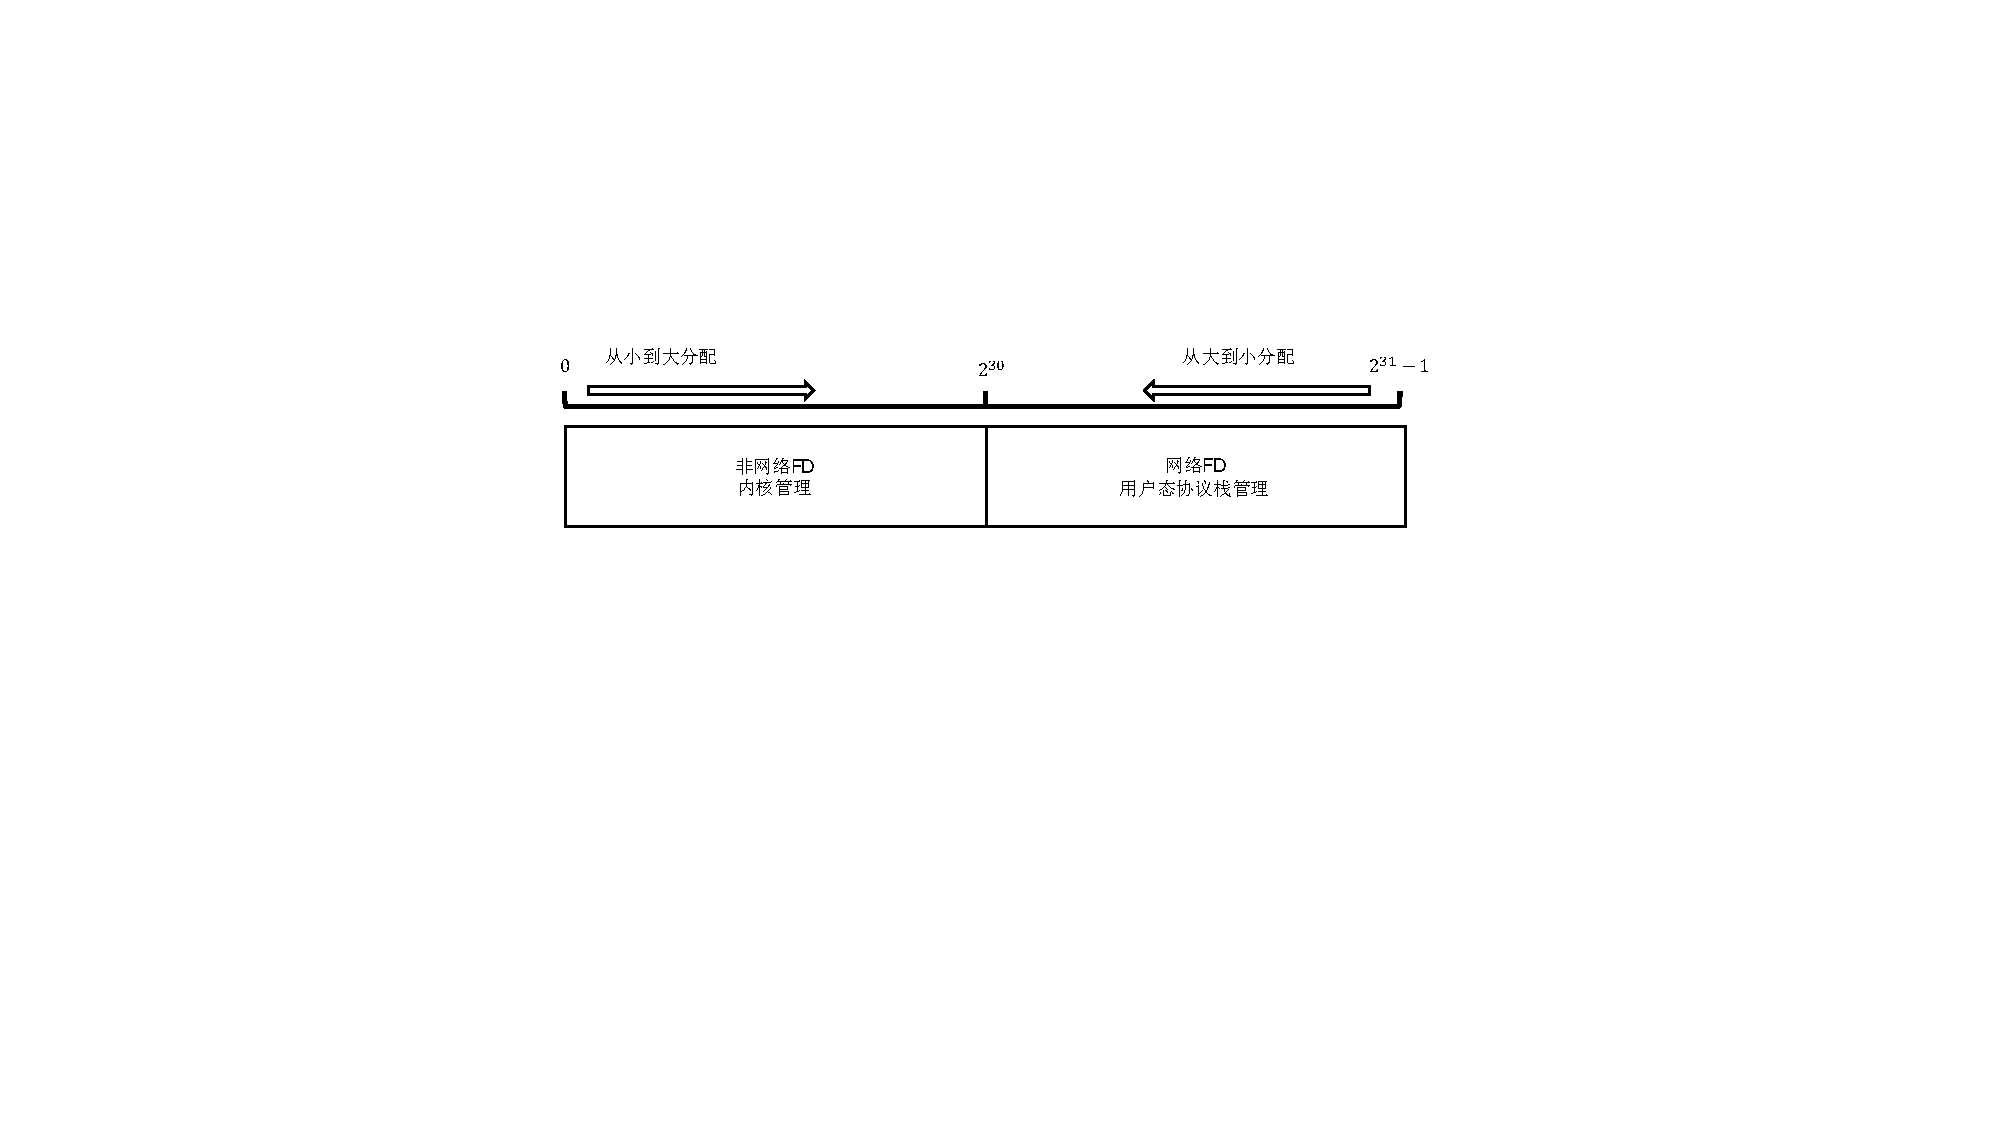
\includegraphics[width=\textwidth]{split_fd1}
  \caption{文件描述符空间管理方案一}
  \label{fig:split_fd1}
\end{figure}
\vspace{-10pt}

为了解决socket文件描述符过大的问题,本文基于资源预分配和双向映射设计了第二种更为科学的文件描述符管理方案。如图~\ref{fig:split_fd2}所示,当用户态协议栈在初始化时会多次调用kernel\_socket函数去申请傀儡文件描述符并放入fd资源池中,这些fd号就提前被该网络应用进程占用,与此同时也会对socket资源提前进行预分配并放入对应的资源池中。当网络应用调用socket或者accept产生一个新连接时,就分别从fd资源池和socket资源池中获取相应的真实fd和协议栈socket数组下标,并建立两者的双向映射关系,方便互相索引查找。当该socket连接关闭的时候,再将真实fd和socket协议栈资源回收,并将双向映射关系重置。这样返回给网络应用的socket fd就是比较小的整数,解决了数组越界访问的问题。
\vspace{-10pt}
\begin{figure}[H] % use float package if you want it here
  \centering
  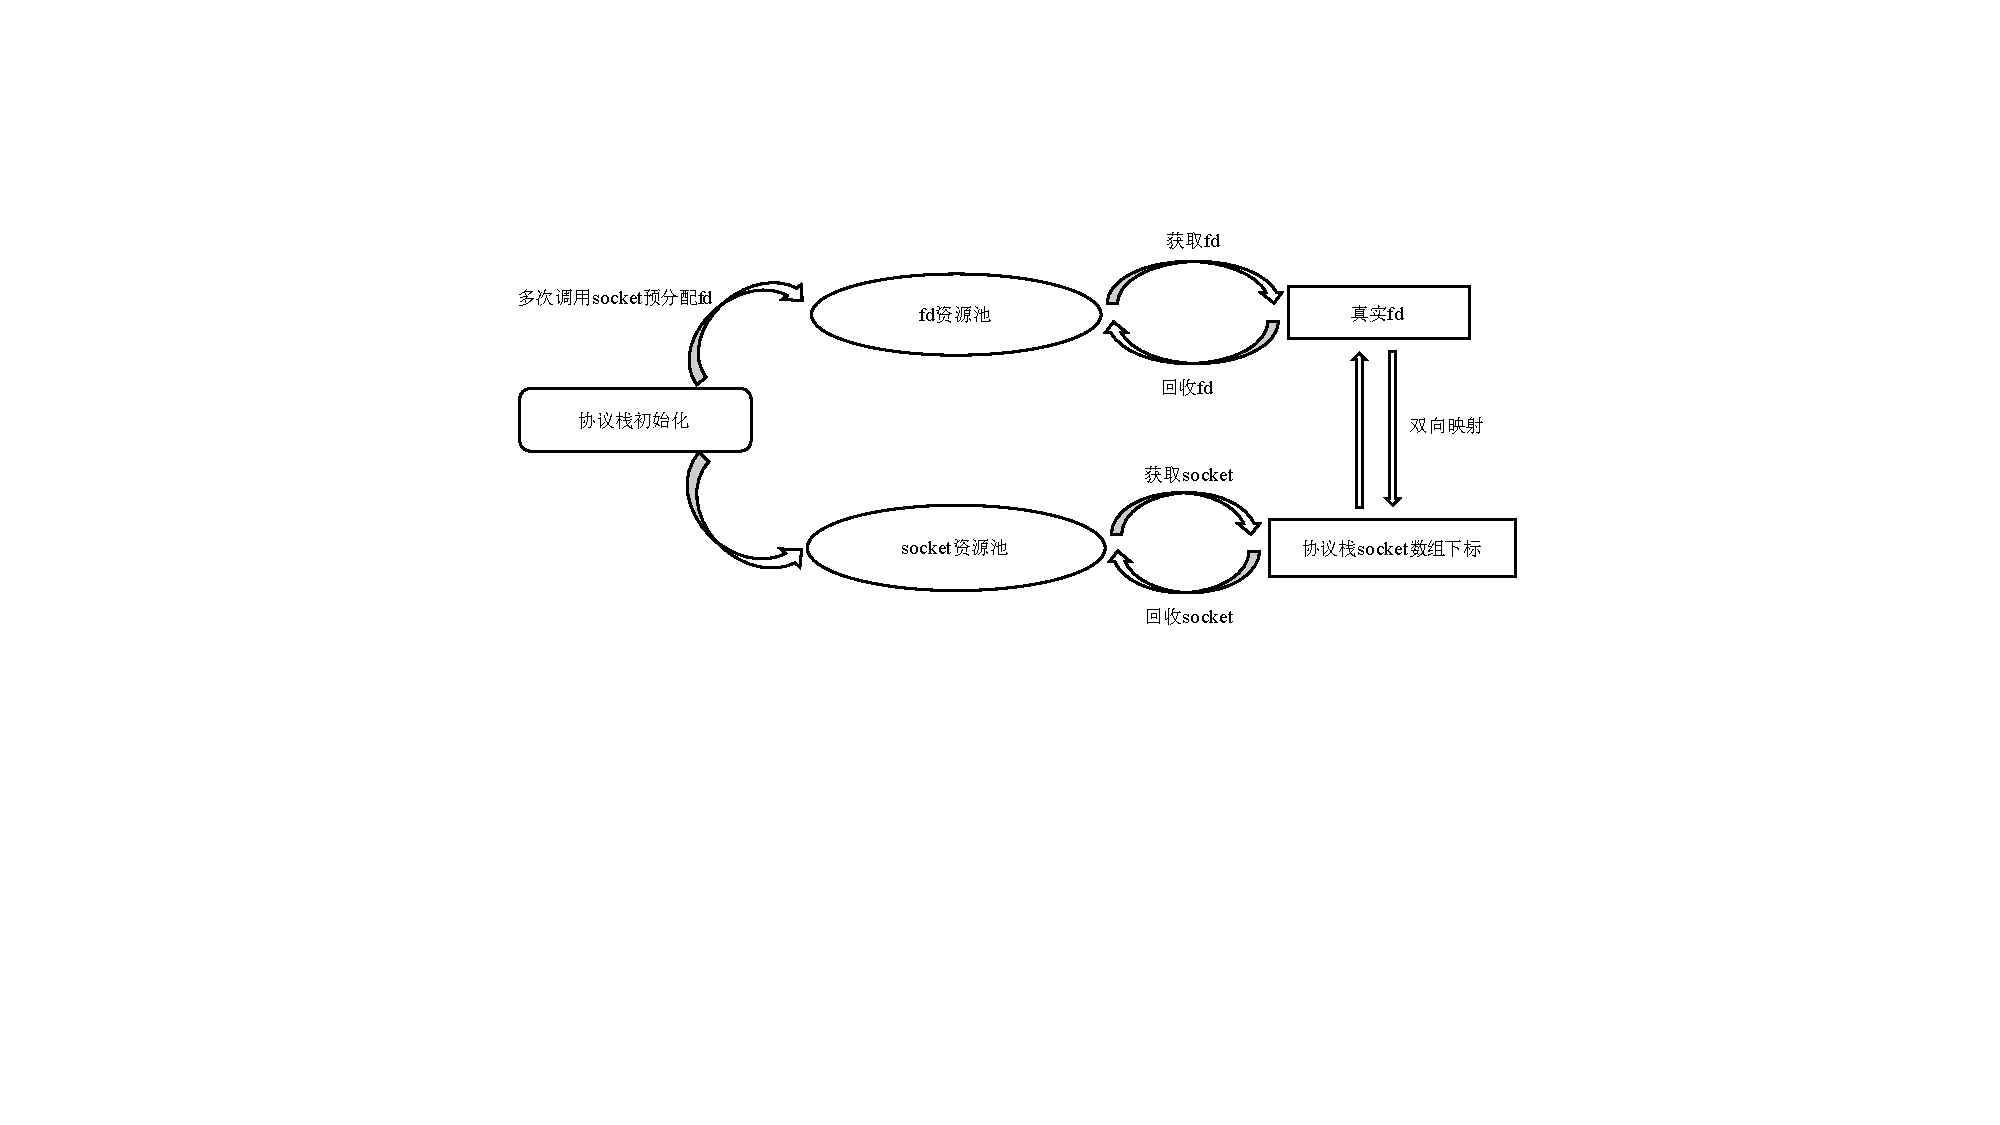
\includegraphics[width=\textwidth]{split_fd2}
  \caption{文件描述符空间管理方案二}
  \label{fig:split_fd2}
\end{figure}
\vspace{-10pt}

此外,资源预分配也降低了新建网络连接时候资源分配的成本以及性能损耗,不过由于预分配的资源有限,一旦网络并发数过大超过资源上限,就必须再分配足够的资源重新放入资源池,否则将出现新建连接失败的情况。所以本系统也为fd和socket资源池设计动态伸缩方案,当资源池剩余资源个数低于总资源数量的10\%将通过Unix域socket通知异常检测模块,并再分配足够的资源放入资源池当中。当资源池中剩余资源个数高于总数的90\%、资源池总数高于初始值且维持该状态超过两分钟之后,也通知异常检测模块将一部分资源进行回收。选取两分钟的时间是因为HTTP长连接的时间大多1分钟左右。资源池的动态伸缩也将在系统异常检测机制一节进行更加详尽的阐述。

\subsection{Epoll IO多路复用的设计}

IO多路复用技术可以让高并发网络连接可以在一个执行流中实现,Linux系统中常见的IO多路复用技术包括poll、select、epoll。前两者的效率较低并且支持的并发连接数有限,而epoll的出现在一定程度上解决传统网络中的C10K问题,这主要得意于epoll在内核中利用在高速缓冲区建立的红黑树和就绪链表数据结构分别表示监听事件和已就绪事件,每次返回给网络应用都是已就绪事件集合,大大降低网络高并发时候的开销。也正是因为epoll的效率之高,所以它在传统网络应用Nginx、Lighttpd、Redis中等被广泛应用。在用户态实现高效的epoll事件监听通知机制就成为该用户态协议栈兼容这些主流网络应用的关键。

在数据结构设计上,用户态协议栈的epoll借鉴内核epoll的设计,采用了红黑树这种高效的平衡二叉搜索树,其可以在$log(n)$时间复杂度内完成结点的插入、查找和删除操作,这在网络并发很高时候作用较大。不过,当网络并发较小的时候,红黑树这种较为复杂的数据结构性能反而不高,所以设计上采用双向链表和红黑树结合的数据结构来表示某个epoll结构体监听事件集合,当网络并发较小的时候采用双向链表,当并发数增加之后就将双向链表转换成红黑树从而加速高并发时网络处理。

在完成数据结构方面的设计之后,用户态协议栈的epoll依然有两个关键技术难点需要解决。第一个难点是如何对socket网络事件和非网络事件同时实现监听与响应,第二个难点是在用户态如何判断有事件已经就绪并返还给网络应用。在用户态由于控制权限较低无法直接对进程的状态进行调度,最简单的思路就是另起一个线程对就绪事件进行不断轮询,一旦轮询到有事件待响应就返回给网络应用。但这种方式对CPU资源的消耗过大,而本协议栈主要通过有名管道和内核epoll解决如上的问题,具体用户态epoll整体架构图如图~\ref{fig:epoll}所示,整个用户态epoll流程分为以下几个步骤:

\begin{enumerate}[(1),labelsep=.5em, leftmargin = 0pt, itemindent = 3em]
\item 当网络应用调用用户态epoll\_create时,前端从epoll资源池中获取一个用户态epoll结构体,并对其进行初始化。初始化过程包括对用户态epoll的双向链表监听结构体进行初始化以及通过kernel\_epoll\_create创建一个内核epoll结构体和有名管道FIFO,并用内核epoll对该FIFO的可读事件进行监听,最终返回给网络应用一个预分配的epoll文件描述符。
\item 当网络应用调用用户态epoll\_ctl时,前端会对被监听文件描述符进行判断,如果是非网络文件描述符,则调用内核epoll\_ctl用内核epoll来操作该事件;而如果是网络文件描述符,对于添加事件操作则将该事件添加到用户态epoll的双向链表结构体中,并在事件数量超过某一阈值后将双向链表转换成红黑树,其他修改、删除操作也是类似。

\vspace{-10pt}
\begin{figure}[H] % use float package if you want it here
  \centering
  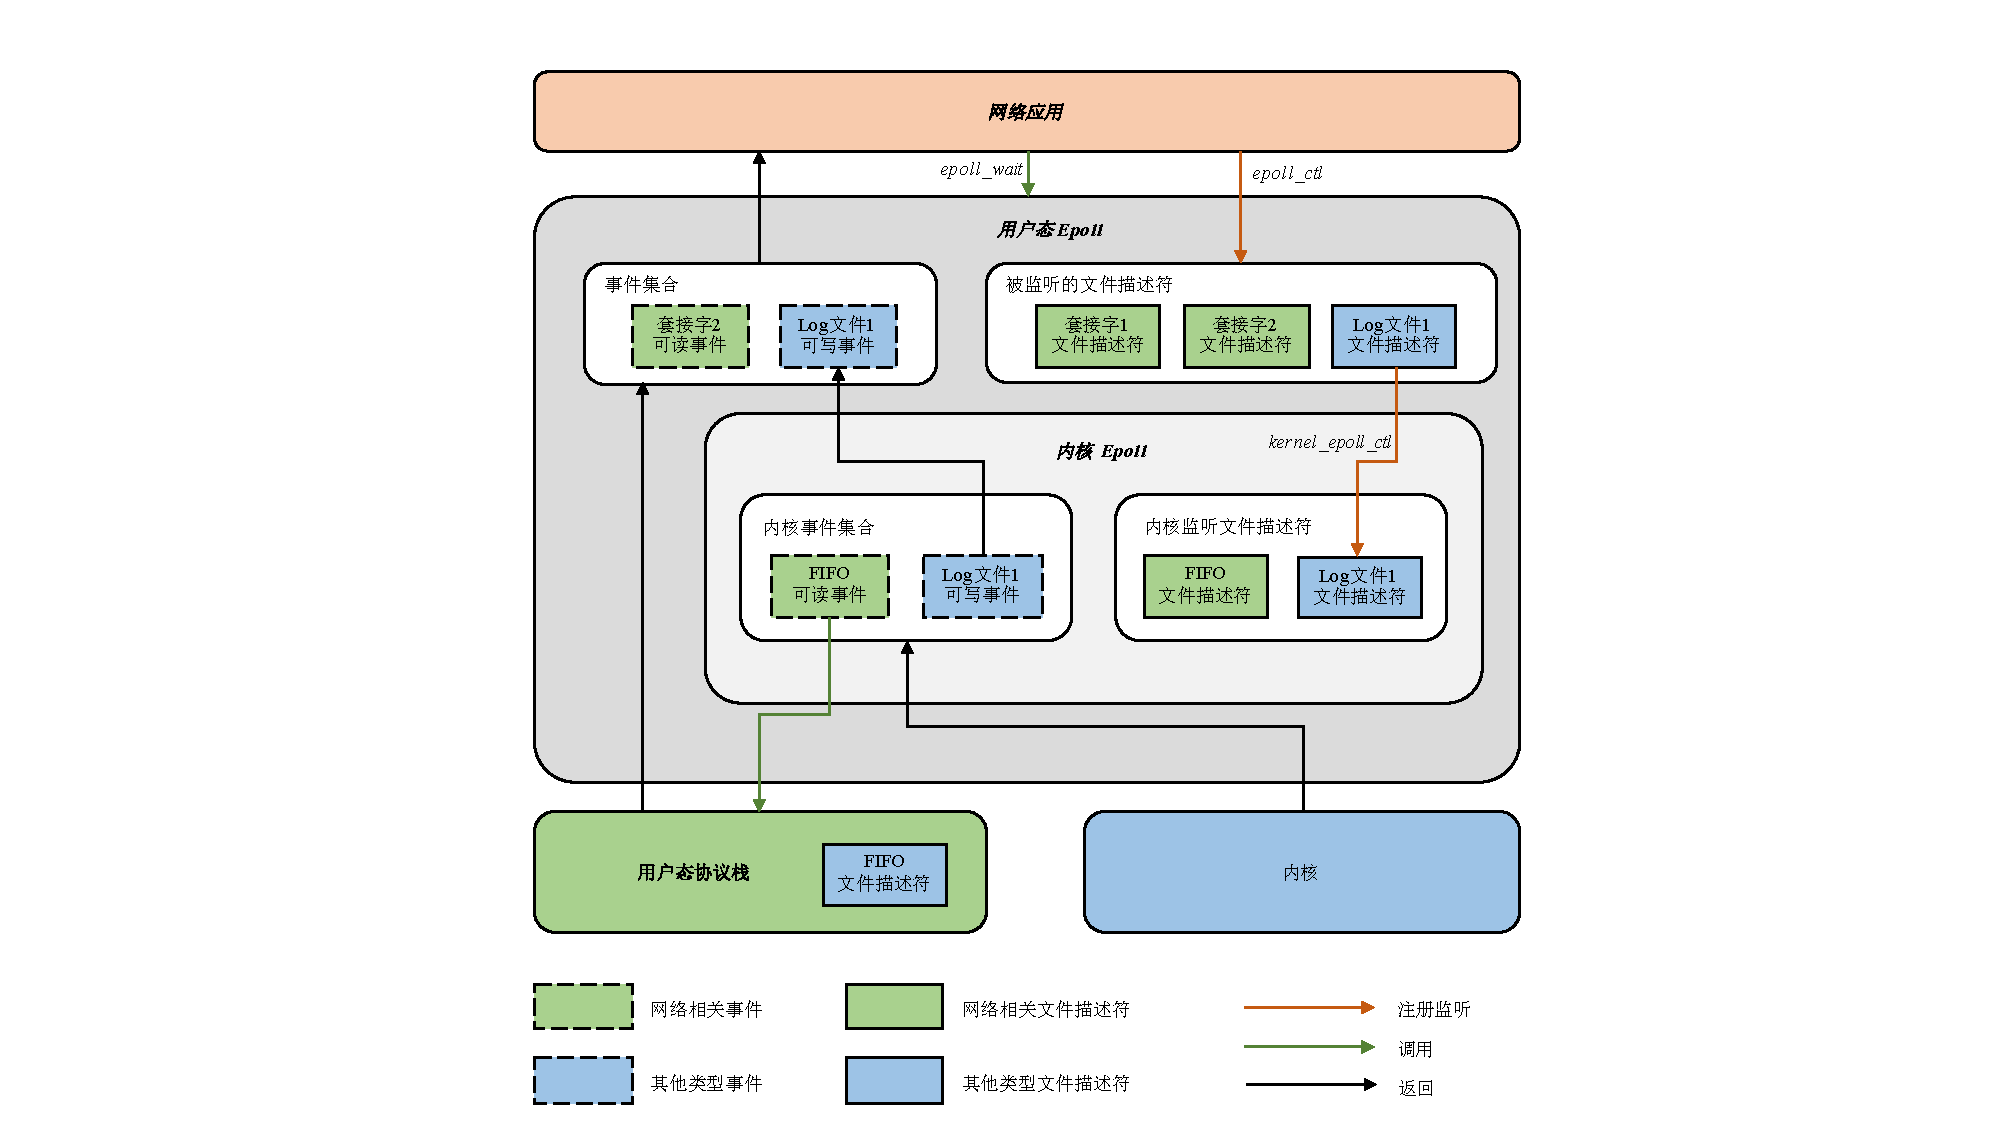
\includegraphics[width=\textwidth]{epoll}
  \caption{用户态epoll设计图}
  \label{fig:epoll}
\end{figure}
\vspace{-10pt}

\item 当网络应用调用用户态epoll\_wait时,会根据timeout参数判断该调用是阻塞还是非阻塞的,如果timeout为0则直接从用户态epoll就绪事件消息队列中获取事件并返回给网络应用,如果timeout大于0则会调用内核epoll\_wait进入休眠阻塞,此时内核epoll同时监听FIFO可读事件和应用注册的非网络事件。
\item 当后端接收到新建连接的、socket的可读可写等事件之后,将这些事件进行聚合,并批量地传递到用户态epoll的就绪事件消息队列中,再向其FIFO写一个字节数据,这样对应的kernel\_epoll\_wait就会被唤醒。此外,非网络事件通过内核渠道的事件触发以及timeout时间到达均可唤醒kernel\_epoll\_wait。
\item 当kernel\_epoll\_wait被事件唤醒之后,便将对应FIFO中的数据全部读出来,并对网络就绪事件消息队列进行全部出队操作,并与内核epoll监听的非网络事件进行聚合,于是网络事件和非网络事件就统一起来返回给网络应用,并等待着下一轮的用户态epoll\_wait调用。
\end{enumerate}

通过以上的设计,用户态epoll就解决了同时对网络文件描述符与非网络文件描述符的事件监听问题,并能在尽可能少占用CPU资源的前提下及时唤醒用户态epoll\_wait并返回给网络应用待响应的事件。

\subsection{并发流网络模型的设计}

在IO多路复用之前,网络服务器在accept出一个新连接后需要创建一个新进程或者线程来对新连接进行读写处理,在连接关闭之后进程或线程就退出,进程或线程不断的产生与销毁对于服务器性能产生过多的损耗。于是在内核网络协议栈陆续推出了poll、select、epoll,其中epoll由于高效的网络并发处理能力而被广泛应用于当下的网络服务器中。然而随着CPU硬件向多核架构方向不断发展,并发执行流结合IO多路复用开始成为当前多种主流网络服务器采用的网络模型。比如Nginx网络服务器可配置成多进程工作模式,如图~\ref{fig:nginx_multiprocess}所示,master进程在完成listen socket的创建之后调用fork产生多个worker进程,多个子进程worker同时监听一个listen socket,并由worker子进程循环调用epoll\_wait监听事件进行网络处理,整个网络服务器master仅负责对worker子进程的监控与管理,而所有网络连接请求的处理由worker进程来完成。Lighttpd也有着与Nginx几乎一样的多进程模式,而像是memcached则是IO多路复用与多线程结合的网络模型。本用户态网络协议栈由于采用协议栈进程与网络应用进程分核的设计,并且协议栈底层使用DPDK轮询IO模式收包占用较多的CPU资源,所以合理对网络应用并发流进行CPU资源和协议栈资源的调度减少或尽量避免CPU资源的争抢是并发流网络模型设计的关键。

\vspace{-10pt}
\begin{figure}[H] % use float package if you want it here
  \centering
  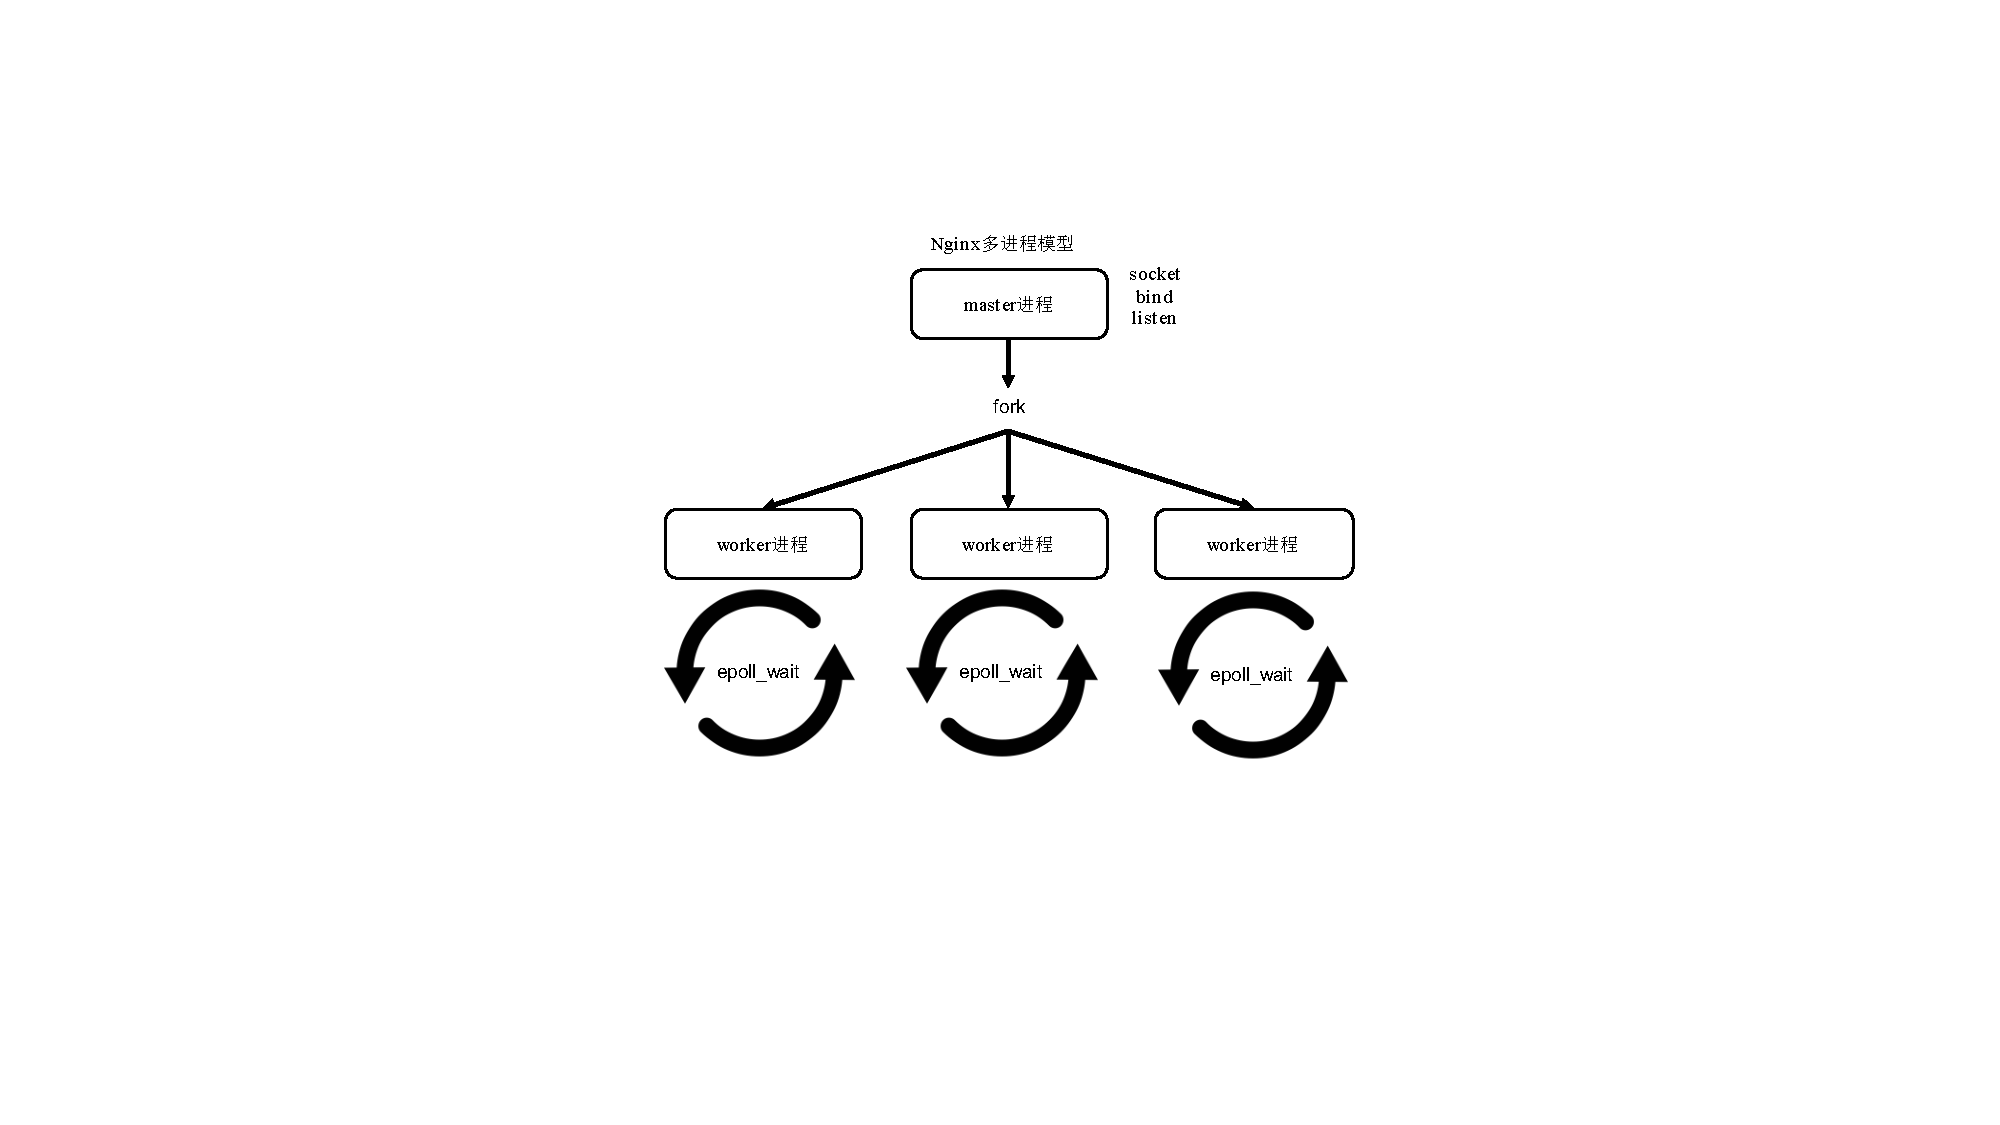
\includegraphics[width=\textwidth]{nginx_multiprocess}
  \caption{Nginx多worker工作模型}
  \label{fig:nginx_multiprocess}
\end{figure}
\vspace{-10pt}

本工作利用DPDK的亲核性通过修改启动脚本将多个协议栈进程分别绑定在专用的CPU核资源上,作为网络事件的生产者进行网络数据包的接收与发送以及网络协议的处理。而对于网络应用执行流(包括进程或线程),则需要为每个执行流分配合适的CPU核与为其提供网络服务的协议栈进程,所以将CPU与提供网络服务的协议栈进程抽象为资源池,CPU资源池可以根据用户配置来决定系统中哪些可用的CPU核作为运行网络服务执行流的资源,而默认配置则将除了协议栈进程占用的CPU核均作为资源池,资源池中资源的获取依据最少服务原则。

对于多进程worker网络模型,当应用调用被劫持的fork函数产生子进程后,依据最少服务原则从CPU资源池中选取其中一个进行亲核性设置,即运行网络应用执行流个数最少的那个CPU会被选定,协议栈进程也根据同样的原理进行选定,并将该子进程worker与选取后的协议栈进行绑定,组成一个协议栈与worker进程对,即该应用进程所有的网络连接最后都在指定的协议栈进程进行处理。由于子进程的地址空间与父进程根据Copy on Write原则相互独立的,并且网络应用中经常出现子进程中关闭父进程中socket fd的情况,所以本系统也为用户态协议栈引入了与内核类似的socket引用计数机制,即fork之后父进程的用户态socket的引用计数自增,在子进程调用用户态close之后只将用户态协议栈管理的引用计数减1,只有当其引用计数减为0之后才真正关闭用户态socket并回收相关资源的操作。对于多线程网络模型的支持,整体与多进程模型相似,主要也是根据最少服务原则为该线程选取CPU核以及协议栈进程。但线程之间不存在文件描述符资源共享的问题,所以也不需要在线程新创建与退出时操作用户态socket的引用计数。除此之外,网络应用进程或线程异常退出时也要将socket和文件描述符资源返还给资源池,防止资源内存泄漏,具体实现会在系统异常检测设计一小节进行详细阐述。

\subsection{系统异常检测设计}

网络服务器应用常作为后台守护进程驻留在系统中一直运行,所以必须防止可能发生的内存泄漏从而避免应用消耗大量宝贵的物理内存资源。这就需要专门的异常检测模块来对网络应用进程进行监控,一旦发生异常崩溃退出后可回收其套接字和文件描述符资源。一些主流网络服务器比如Nginx会对worker异常退出进行监控并重启创建新的worker,但用户态套接字等资源还需要由用户态协议栈来管理。

\vspace{-10pt}
\begin{figure}[H] % use float package if you want it here
  \centering
  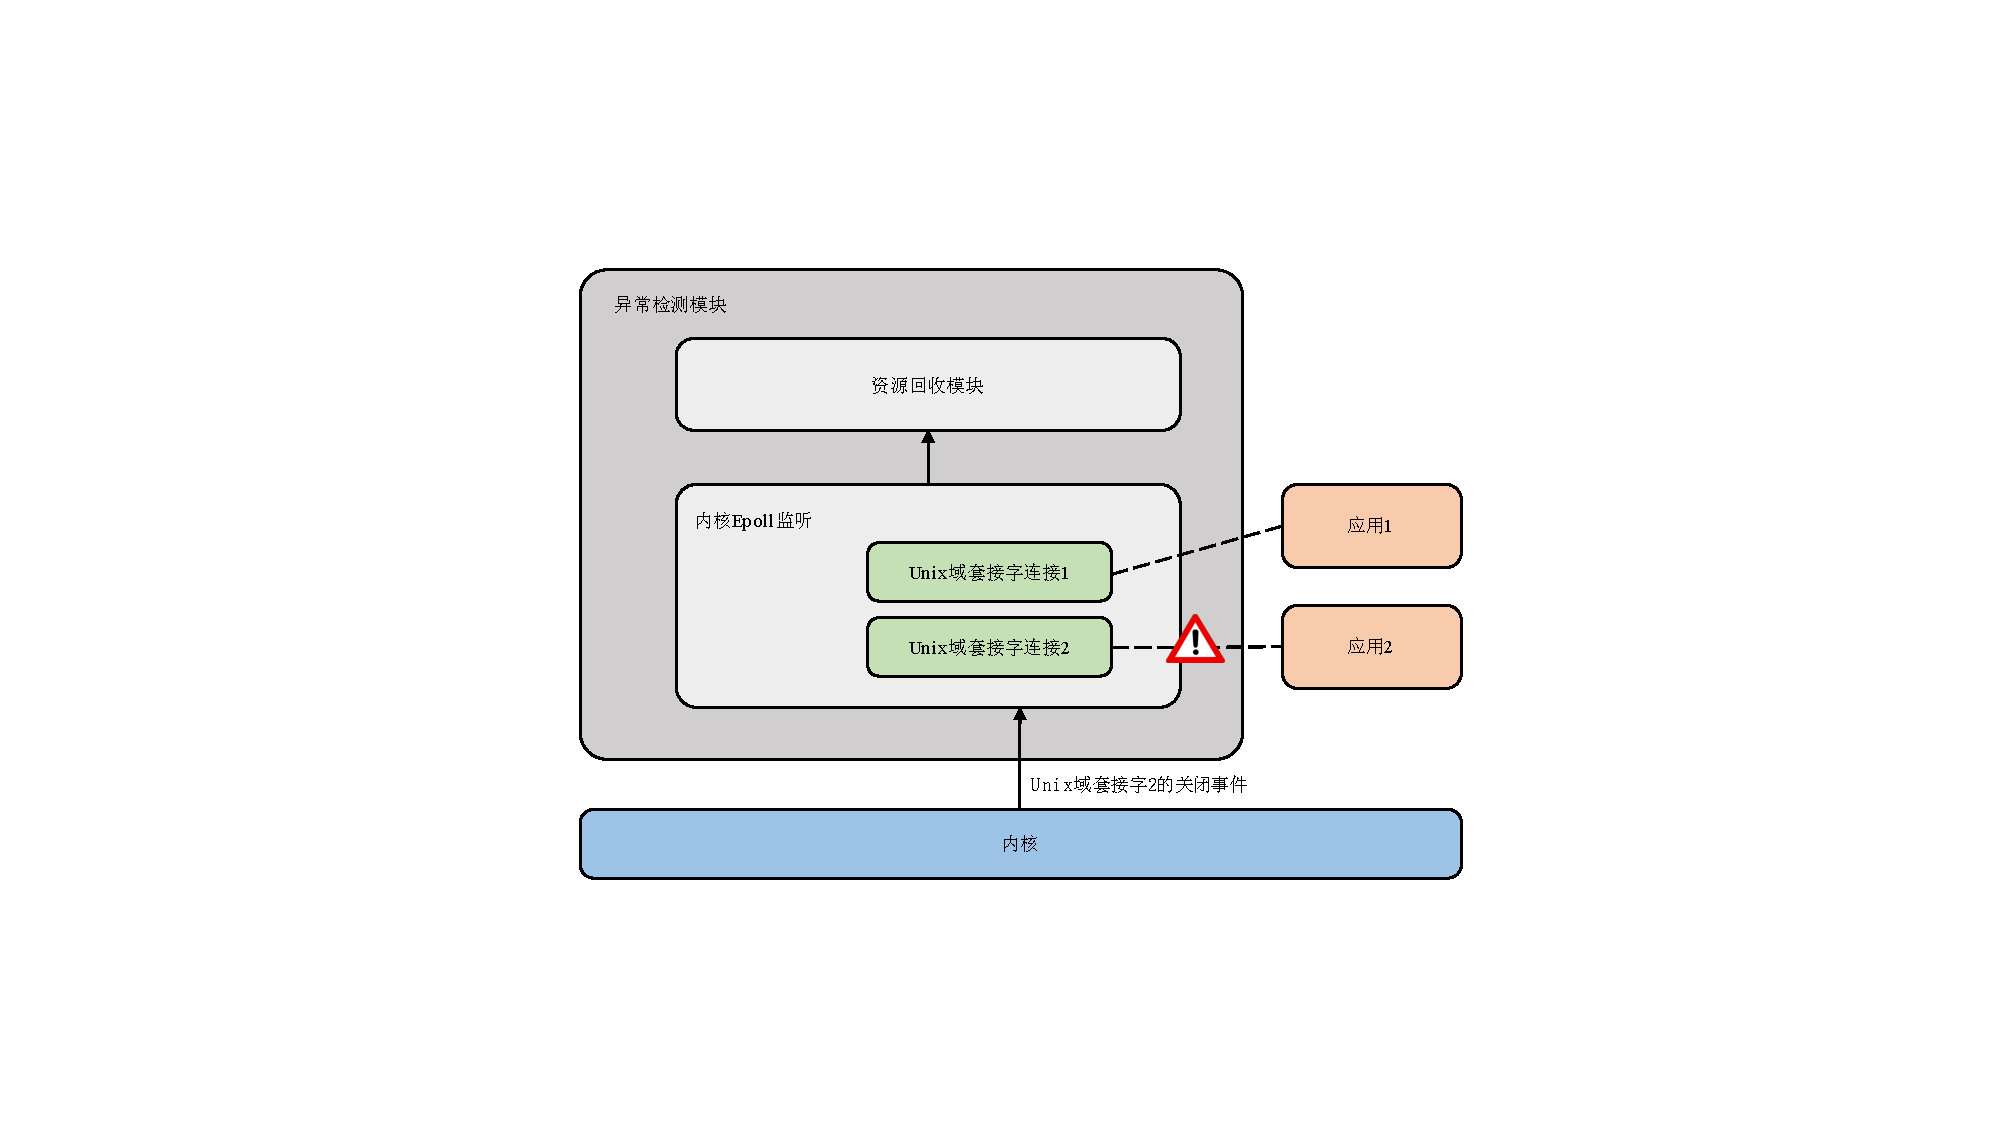
\includegraphics[width=\textwidth]{exception}
  \caption{异常检测模块设计图}
  \label{fig:exception}
\end{figure}
\vspace{-10pt}

异常检测模块的核心是Unix域套接字并利用内核套接字在进程崩溃退出之前会向对端发送FIN包的机制,整个模块的设计思路如图~\ref{fig:exception}所示,当用户态协议栈初始化时会创建一个监听Unix域套接字,在某端口等待本地其他套接字的连接,并用内核epoll监听该Unix域套接字的EPOLL\_CTL\_DEL事件。而当网络应用动态链接到用户态协议栈进行初始化时会创建一个主动连接的内核套接字,调用connect函数与本地Unix域监听套接字建连,这样就在网络应用进程与其对应的用户态协议栈进程中建立套接字通信管道。当网络应用进程崩溃后,其内核套接字会自动向Unix域监听套接字发送FIN包关闭该连接,而用户态协议栈后端在轮询中会定期检查异常检测模块中的内核epoll事件,当协议栈进程收到该FIN包后,协议栈异常检测模块的epoll\_wait返回EPOLL\_CTL\_DEL事件,并根据其文件描述符确定哪个应用异常退出,接下来会将这些信息传递到资源回收模块,对用户态套接字和文件描述符资源进行回收。

该机制对于网络应用线程异常崩溃是无法生效的,因为内核文件描述符在进程地址空间被多个线程共享,即使一个线程退出,也不会触发该内核文件描述符向对端发送FIN包。而对于线程池类型的服务,一个线程由于常驻系统中,对其管理的资源进行回收也是很有必要的。而本系统利用pthread\_cleanup\_pop、pthread\_cleanup\_push函数并对pthread\_create函数进行接管,再次封装其主回调函数并将资源回收的相关函数加入pthread的cleanup栈中,这样当该线程异常退出后,便会执行该资源回收回调函数。这样便可完成网络应用线程的异常退出资源回收。不过该方案对于thread per request多线程模型代价过大,而每新来一个连接便创建一个线程来处理,这种短生命周期的线程由于发生异常崩溃的几率很小,所以该机制对于短生命周期的执行流可根据用户配置进行关闭。